\documentclass{article}
% ВНИМАНИЕ: Используйте LuaLatex для сборки этого документа
\usepackage{expl3,xargs,comment,enumitem,subcaption,graphicx,float}
\usepackage{amsmath,amssymb,mathtools}
\usepackage[margin=2cm]{geometry}
\usepackage{alltt, xcolor,fontspec,luacode,polyglossia}
\setdefaultlanguage[spelling = modern]{russian}
\setotherlanguage{english}
\setmainfont{CMU Serif}
\setsansfont{CMU Sans Serif}
\setmonofont{CMU Typewriter Text}
\usepackage[unicode]{hyperref}
\usepackage{tikz}
\usetikzlibrary{fadings,scopes,decorations}
\usetikzlibrary{decorations.pathreplacing}
\usetikzlibrary{angles,calc,quotes,positioning}
\usepackage{pgfplots,unicode-math,wasysym}
\usepackage{minted}
%\usepackage[outputdir=build]{minted}
% ВНИМАНИЕ: УДАЛИТЕ [outputdir=build], если сборка идет в корневой директории, иначе будут ошибки.
% ВНИМАНИЕ: Команда для сборки в директории build:
% lualatex -synctex=1 -shell-escape -output-directory=build -interaction=nonstopmode %.tex
\usepackage{enumitem}
\def\pr<#1>{\input{#1}}
\def\lasttiming{0}

\begin{document}
	\tableofcontents
	\newcommand\cmd[1]{\colorbox{gray!20}{\texttt{#1}\phantom{/}\!\!\!\!}}

\section{Базовый синтаксис}

Про язык Perl существует миф, что это write-only язык.
На самом деле, если текст понимает интерпретатор, то сможет прочесть и человек.
Цель этой лекции~--- научить читать исходные тексты практически любой программы.

Основная идея, лозунг Perl~--- есть более одного способа сделать что-либо в этом языке (\textit{TIMTOWTDI}, \textit{There's More Than One Way To Do It}).
При написании программы стоит следовать пути удобочитаемости ее текста.
К сожалению, не все придерживаются этого принципа, и зачастую прочесть программу может лишь интерпретатор Perl: \textit{the only thing can parse Perl (the language) is perl (the binary)}.

\subsection{Условия и циклы} 
Одной из простейших конструкций является \textit{блок}~--- ограниченный фигурными скобками код.
Внутри блока размещаются несколько раздельных \textit{statement}:

%00:02:06
\pr<code/L01_code_001.pl>

При этом блок \o{do} не является блоком, а является единичным \textit{statement}.
В отличие от блока, то, что написано в фигурных скобках \textit{do}, возвращает свое значение:

%00:02:06
\pr<code/L01_code_002.pl>

Блок используется в существующих конструкциях для создания отдельных областей видимости.

\subsection{Управляющие функции}
Для управления циклами существует управляющая конструкция \textit{next}.
В языке Си есть аналог \textit{continue}.
При этом \textit{next} можно вызвать в любом месте тела цикла, при этом исполнение перенесется в начало блока \textit{continue} цикла.
Если такого блока нет, то исполнение перенесется в конец тела и перейдет на следующую итерацию:

%00:02:52
\pr<code/L01_code_003.pl>

Команда \textit{last} позволяет выйти из цикла и прекратить его исполнение без выполнения блока \textit{continue}.
В следующем примере показан цикл \textit{for}, но на его месте может быть любой цикл~--- \textit{while}, \textit{until} и другие:

%00:03:31
\pr<code/L01_code_004.pl>

В языке Си аналогом \textit{last} является оператор \textit{break}.

%Переменная состояния - слова лектора
Команда \textit{redo} начинает итерацию цикла~--- переходит в начало цикла без изменения переменной состояния.
Если просто написать внутри цикла \textit{redo}, то получится бесконечный цикл, так как он не изменяет никакие переменные.
В некоторой степени это аналог оператора \textit{goto} в Си:

%00:03:52
\pr<code/L01_code_005.pl>

Еще одна особенность блока заключается в том, что любой пустой блок идентичен циклу с одной итерацией.
В таком блоке работают вызовы \textit{redo}, \textit{last}, \textit{next}.
Оператор \textit{redo} идет в начало блока, \textit{last} выходит из блока, а \textit{next} переходит в конец блока:

%00:04:14
\pr<code/L01_code_006.pl>

В языке Perl существует оператор выбора \textit{given/when} (аналог \textit{switch/case} из Си).
Внутри~--- не обычный \textit{case}, а довольно сложный оператор \textit{smart match}.
Внутри \textit{when} можно писать разные выражения:

%00:04:33
\pr<code/L01_code_007.pl>

В отличие от других языков, здесь нет ключевого слова \textit{break}~--- \textit{break} автоматически подразумевается внутри каждого условия \textit{when}.
Для <<проваливания>> в другой \textit{when} используется \textit{continue}.

В языке Perl есть определенные функции и операторы, которые имеют множественное поведение.
Один из примеров~--- \textit{goto}, используемый для перехода.
Данный оператор является классическим, и, как и в других языках, выполняет переход на метку:

%00:05:32
\pr<code/L01_code_008.pl>

Метка записывается статически, она объявлена в программе.

Существует также устаревший синтаксис, использовать который не рекомендуется.
Здесь в качестве параметра \textit{goto} можно передать строку, а имя строки будет воспринято как метка:

%00:06:04
\pr<code/L01_code_009.pl>

\textit{Хвостовой вызов} позволяет вызвать тело другой функции на месте этой функции с теми аргументами, которые есть сейчас (\textit{goto}~$\&$).
В следующем примере показано классическое написание функции вычисления чисел Фибоначчи, которая делает рекурсивный вызов:

%00:06:30
\pr<code/L01_code_010.pl>

Известная проблема с рекурсией заключается в том, что у нее растет стек.
Если же заменить строку вызова функции на выражение, показанное в следующем примере, то эта функция будет выполнена непосредственно на данном месте (без создания отдельного \textit{stack frame}):

%00:07:36
\pr<code/L01_code_011.pl>

Аналогичным образом можно написать расчет факториала.
Функция также написана в рекурсивном стиле, но при этом она никогда не вызовет переполнение стека.

%00:07:56
\pr<code/L01_code_012.pl>

\subsection{Постфиксная нотация}
Помимо классического написания условий и циклов, в языке Perl возможна \textit{постфиксная нотация}.
Она подразумевает, что \textit{statement} выполнится независимо от того, выполняется условие или нет:

%00:08:15
\pr<code/L01_code_013.pl>

Постфиксная нотация используется, когда \textit{statement} в приложении важнее чем то, что идет после него.
Так можно обратить внимание того, кто читает программу, на то, что именно сейчас выполняется.
Постфиксная нотация может использоваться внутри \textit{given/when}.

Так как \textit{do} является \textit{statement}, то можно после него написать любой из блоков (\textit{while}, \textit{until}, \textit{for}, \textit{if}):

%00:08:15
\pr<code/L01_code_014.pl>

Это выглядит как постфиксный цикл, но у него есть определенная особенность: не работают все функции управления циклом, так как эти операторы работают внутри блока.

\renewcommand{\lasttiming}{580}
\section{Переменные} %00:09:39:00 - Переменные (основные типы, ссылки, интерполяция)

\subsection{Основные типы}
Любой идентификатор переменной записывается следующим образом.
Значком, который называется \textit{Sigil}, может быть один из пяти символов:~$\$, @, \%, \&, ^{\ast}$ (см.~рис.~1).
Символ~$\$$ означает скалярный контекст или скалярную переменную, символ~$@$~--- либо массив, либо списковый контекст.
Символ~$\%$ относится к хэшу, символ~$\&$~--- к блоку кода (к указателю на функцию).
Символ~$^{\ast}$ означает специальный тип \textit{glob}.

%Рис. 1: 00:09:53
\begin{figure}[h!]\center
	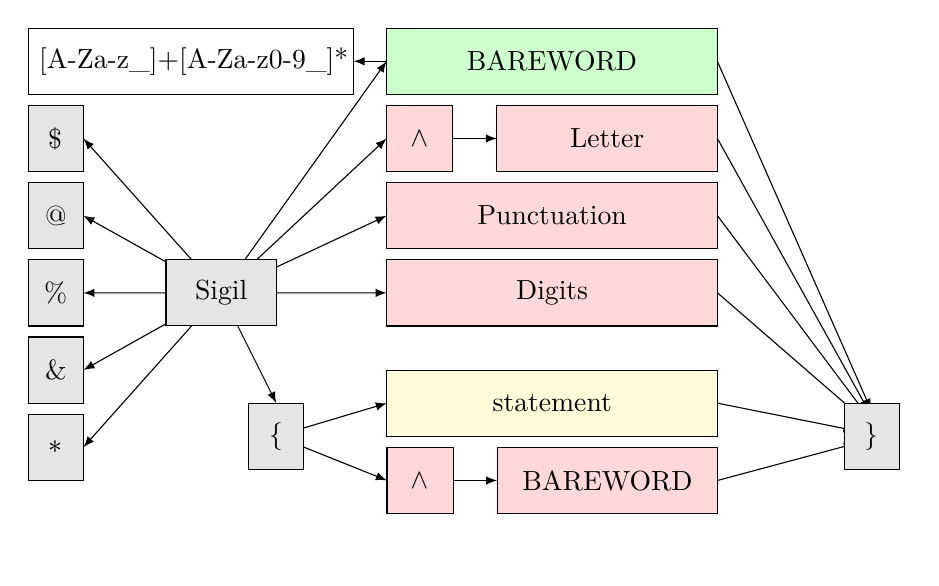
\begin{tikzpicture}[scale=1.4] \def\setpoints#1(#2)#3<#4,#5>#6 at (#7);{
		\path[shift={(#7)}]
		( 0     , 0      ) coordinate (#2)
		( 0.5*#4, 0      ) coordinate (#2_east)
		( 0     , 0.5*#5 ) coordinate (#2_north)
		(-0.5*#4, 0      ) coordinate (#2_west)
		( 0     ,-0.5*#5 ) coordinate (#2_south)
		( 0.5*#4, 0.5*#5 ) coordinate (#2_north_east)
		(-0.5*#4, 0.5*#5 ) coordinate (#2_north_west)
		( 0.5*#4,-0.5*#5 ) coordinate (#2_south_east)
		(-0.5*#4,-0.5*#5 ) coordinate (#2_south_west); }



\def\doit{\draw[latex-] (box_west) -- (s); \draw[-latex] (box_east) -- (e);}
\def\stepbl{\path (current)+(0,-7mm) coordinate (current);}
\def\dblock<#1>(#2){
		\setpoints (box) <30mm,6mm> at (current);
		\draw[fill={#1}] (box_south_west) rectangle (box_north_east) (box) node {#2};
		\doit\stepbl }
\def\dblockl<#1>(#2){
		\setpoints (box) <30mm,6mm> at (current);
		\setpoints (box_in)  <6mm,6mm> at ($(box_west)+(0.3,0)$);
		\draw[fill={#1}] (box_in_south_west) rectangle (box_in_north_east) (box_in) node {$\wedge$};
		\draw[-latex] (box_in_east) --+ (4mm,0);
		\setpoints (box_in)  <20mm,6mm> at ($(box_west)+(2,0)$);
		\draw[fill={#1}] (box_in_south_west) rectangle (box_in_north_east) (box_in) node {#2};
		\doit\stepbl }
\def\dsmallblock<#1><#2> (#3) at (#4);{ \setpoints (box) <#1> at (#4);
		\draw[fill={#2}] (box_south_west) rectangle (box_north_east);
		\draw (box) node {#3}; }
	
	\def\block#1(#2)#3<#4>[#5] at (#6);{
		\setpoints (#2) <#4> at (#6);
		\draw (#2_south_west) rectangle (#2_north_east) (#2) node {\texttt{#5}};
	}
	
	
%---------------------------------------------

\def\block#1(#2)#3<#4>[#5] at (#6);{
	\setpoints (#2) <#4> at (#6);
	\draw (#2_south_west) rectangle (#2_north_east) (#2) node {\texttt{#5}};
}
\def\arr<#1>{\textcolor{blue}{[}#1\textcolor{blue}{]}}
\def\h<#1>{\textcolor{blue}{\{}#1\textcolor{blue}{\}}}
\def\curv<#1>{\textcolor{red}{\{}#1\textcolor{red}{\}}}
\def\red|#1|{\textcolor{red}{#1}}	
\path (0,0) coordinate (current) 
	  (1.5,-2.1) coordinate (s) 
	  (7.5,-3.4) node[circle] (e) {\}};

	\foreach \n in {$\$$,$@$,$\%$, $\&$, $*$} {\stepbl
		\dsmallblock<5mm,6mm><gray!20> (\n) at (current);
		\draw[latex-] (box_east) -- (s);	}
	\path (4.5,0) coordinate (current);
	\dblock<green!20>(BAREWORD)
	\draw[-latex] (box_west) --+ (-3mm,0);
	\draw (box_north_west) + (-3mm,0) rectangle ($(box_south_west)+(-32.5mm,0)$);
	\draw (box_west) + (-17.5mm,0) node{[A-Za-z\_]+[A-Za-z0-9\_]*};
	\dblockl<red!15>(Letter)
	\dblock<red!15>(Punctuation)
	\dblock<red!15>(Digits)
	\path (2,-3.4) coordinate (s) (current)+(0,-3mm) coordinate (current);
	\dblock<yellow!15>(statement)
	\dblockl<red!15>(BAREWORD)
	\dsmallblock<5mm,6mm><gray!20> ($\{$) at (2,-3.4);
	\draw[-latex] (1.5,-2.1) -- (box_north);
	\dsmallblock<5mm,6mm><gray!20> ($\}$) at (7.4,-3.4);
	\dsmallblock<10mm,6mm><gray!20> (Sigil) at (1.5,-2.1);
\end{tikzpicture}
	\caption{Правила составления идентификаторов переменных в Perl}
\end{figure}

После \textit{Sigil} в классическом случае будет идти переменная \textit{Bareword}~--- любое сочетание букв, которое начинается с большой, маленькой буквы или с подчеркивания и продолжается тем же набором плюс цифры.

Вокруг любой конструкции, идущей после \textit{Sigil}, можно поставить фигурные скобки.
Кроме \textit{Bareword}, после \textit{Sigil} может идти спецпеременная.
Таковыми являются:~$\^+ Letter$, единичный элемент пунктуации, цифры.
Внутри фигурных скобок также может быть написан любой \textit{statement}, а также спецпеременная~$\^+Bareword$ (см.~рис.~1).
Примеры обычных переменных:
\begin{itemize}[noitemsep]
	\item \$var, @array, \%hash, \&func, *glob
	\item \$\{var\}, @\{array\}, \%\{hash\}, \&\{func\}, *\{glob\}
	\item \$\{  "scalar"  .  "name"  \}, \%\{  "hash" . \$id  \}
\end{itemize}

Примеры специальных переменных:
\begin{itemize}[noitemsep]
	\item \$\textasciicircum W, \$\textasciicircum O, \$\textasciicircum X, \$\{\textasciicircum W\}, \$\{\textasciicircum O\}, \$\{\textasciicircum X\}, ...
	
	\item \$0, \$1, \$100, \$\{0\}, \$\{1\}, \$\{100\}, ...
	
	\item \$\{\textasciicircum PREMATCH\}, \$\{\textasciicircum MATCH\}, \$\{\textasciicircum POSTMATCH\}, ...
	
	\item \$\_, @\_, \$!, \$@, \$?, \$", \$/, \$, , ...
	
	\item \$\{\_\}, @\{\_\}, \$\{!\}, \$\{@\}, \$\{?\}, \$\{"\}, \$\{/\}, \$\{,\}, ...
\end{itemize}

\textit{Числа} можно записать в Perl различными способами:

%00:13:23
\pr<code/L01_code_015.pl>

Особенность заключается в следующем: в числе можно в любом месте, кроме как рядом с точкой, вставлять подчеркивание.
Это делается исключительно для большей легкости прочтения текста программы, интерпретатор такие подчеркивания пропускает.

\textit{Строки} в Perl бывают привычного вида (в двойных кавычках и в одинарных).
Строки в одинарных кавычках являются неинтерполируемыми, в двойных~--- интерполируемыми.
Строку можно разорвать как угодно:

%00:13:58
\pr<code/L01_code_016.pl>

Внутри двойных кавычек работает интерполяция переменных: любой идентификатор, записанный внутри двойных кавычек, будет развернут в свое значение.
Строку можно собирать при помощи оператора конкатенации из специальных констант.

Особенность строк в языке Perl состоит в следующем.
Если в строке содержится довольно много обычных кавычек, и их использовать неудобно, то можно выбрать любой другой символ для обозначения границы строк.
Оператор \textit{q} отвечает за одинарную кавычку, \textit{qq}~--- за двойную, и далее следует какой-либо разделитель:

%00:13:58
\pr<code/L01_code_017.pl>

Внутри строк с двойной кавычкой поддерживается синтаксис записи~$\backslash x$~--- шестнадцатеричный код юникодного символа.
Так можно записать любой символ, который есть в таблице \textit{Unicode}:

%00:13:58
\pr<code/L01_code_018.pl>

Еще одной особенностью Perl в данном разделе является \textit{v-string}.
Он используется для создания и обозначения версий, для сравнения их между собой.

%00:13:58
\pr<code/L01_code_019.pl>

\subsection{Ссылки}
Помимо чисел и строк, важно также рассмотреть \textit{ссылки}.
Ссылку можно создать при помощи оператора взятия ссылки ($\backslash$) на любой известный объект:

%00:13:58
\pr<code/L01_code_020.pl>

Существуют анонимные конструкторы ссылок на массив (квадратные скобки) и на хэш (фигурные скобки).
Также можно создать анонимную функцию:

%00:13:58
\pr<code/L01_code_021.pl>

Ссылки можно присваивать спискам, причем поставив ссылку на список, можно создать ссылку на все его элементы:

%00:13:58
\pr<code/L01_code_022.pl>

Часто необходимо понять, чем является сложная структура~--- массивом, ссылкой на массив или даже скаляром.
\textit{Sigil} означает контекст обращения, как было показано ранее.
Появляется специальный \textit{Sigil} из двух элементов~$\$\#$, обозначающий последний элемент в массиве.
Далее идет идентификатор (см.~рис.~2).
Если после идентификатора идет квадратная или фигурная скобка, то это либо массив, либо хэш.

%Рис. 2: 00:17:29
\begin{figure}[h!]\center
	\begin{tikzpicture}
\def\setpoints#1(#2)#3<#4,#5>#6 at (#7);{
	\path[shift={(#7)}]
	( 0     , 0      ) coordinate (#2)
	( 0.5*#4, 0      ) coordinate (#2_east)
	( 0     , 0.5*#5 ) coordinate (#2_north)
	(-0.5*#4, 0      ) coordinate (#2_west)
	( 0     ,-0.5*#5 ) coordinate (#2_south)
	( 0.5*#4, 0.5*#5 ) coordinate (#2_north_east)
	(-0.5*#4, 0.5*#5 ) coordinate (#2_north_west)
	( 0.5*#4,-0.5*#5 ) coordinate (#2_south_east)
	(-0.5*#4,-0.5*#5 ) coordinate (#2_south_west);
}



\path (0,0) coordinate (current) (1.25,-2.1) coordinate (s) (7.5,-3.4);

\def\doit{\draw[latex-] (box_west) -- (s); \draw[-latex] (box_east) -- (e);}
\def\stepbl{\path (current)+(0,-7mm) coordinate (current);}
\def\dblock<#1>(#2){
	\setpoints (box) <30mm,6mm> at (current);
	\draw[fill={#1}] (box_south_west) rectangle (box_north_east) (box) node {#2};
	\doit\stepbl }


\def\dsmallblock<#1><#2> (#3) at (#4);{ \setpoints (box) <#1> at (#4);
	\draw[fill={#2}] (box_south_west) rectangle (box_north_east);
	\draw (box) node {#3}; }

\def\block (#1) <#2> [#3] <#4> at (#5);{
	\setpoints (#1) <#2> at (#5);
	\draw[fill=#3] (#1_south_west) rectangle (#1_north_east) (#1) node {\texttt{#4}};
}


\draw (-2.3,0.2) node[below right]{Context} rectangle (1.8,-4.3);

\foreach \n/\l in {$\$$/Scalar,$@$/Array,$\%$/Last elt, $\&$/Hash, $*$/Code} {\stepbl
	\dsmallblock<5mm,6mm><gray!20> (\n) at (current);
	\draw[latex-] (box_east) -- (s); 
	\draw (box_west)+(-1cm,0) coordinate (temp);
	\dsmallblock<15mm,6mm><gray!20> (\l) at (temp);
	\draw[latex-] (box_east) --+ (0.25cm,0); }


\foreach \place/\up/\down/\n/\name in {(5cm,-0.5cm)/Digits/Stmt/up/Array|ArrayRef,(5cm,-4cm)/BareW/Stmt/down/Hash|HashRef}{
	\begin{scope}[shift={\place}]
	\draw (-0.3, 1.3) node[below right]{\name }  rectangle (3.3,-1);
	\path (0,0) coordinate (current);
	\block (l\n) <4mm,6mm> [red!20] <[> at (current);
	\block (r\n) <4mm,6mm> [red!20] <]> at ($(current)+(3,0)$);
	\block (u\n) <14mm,6mm> [gray!20] <\up> at ($(current)+(1.5, 0.4)$);
	\block (d\n) <14mm,6mm> [gray!20] <\down> at ($(current)+(1.5,-0.4)$);
	\begin{scope}
	\draw[-latex] (l\n_east) -- (u\n_west); 
	\draw[-latex] (l\n_east)+(0,-0.1) -- (d\n_west); 
	\draw[latex-] (r\n_west)+(0, 0.1) -- (u\n_east); 
	\draw[latex-] (r\n_west)+(0,-0.1) -- (d\n_east); 
	\end{scope}
	
	\end{scope}}

\dsmallblock<10mm,6mm><gray!20> (Sigil) at (1.2,-2.1);
\draw[-latex] (box_east)--+(0.3cm,0);
\dsmallblock<10mm,6mm><green!20> (ID) at (2.5,-2.1);
\draw[-latex] (box_east)--+(0.3cm,0);
\draw[-latex] (box_north)--(lup_west); \draw[-latex] (box_south)--(ldown_west);
\dsmallblock<10mm,6mm><green!20> (\texttt{->}) at (3.8,-2.1);
\draw[-latex] (box_north)--(lup_south); \draw[-latex] (box_south)--(ldown_north);

\end{tikzpicture}

	\caption{Правила записи массивов и хэшей}
\end{figure}

Если же после идентификатора идет стрелка (оператор разыменования ссылки), то после него опять же может идти либо квадратная, либо фигурная скобка.
Это означает, что в идентификаторе лежит ссылка~--- существует переменная, которая является ссылкой на массив или на хэш (см.~рис.~3).

%Рис. 3: 00:17:29
\begin{figure}[h!]\center
	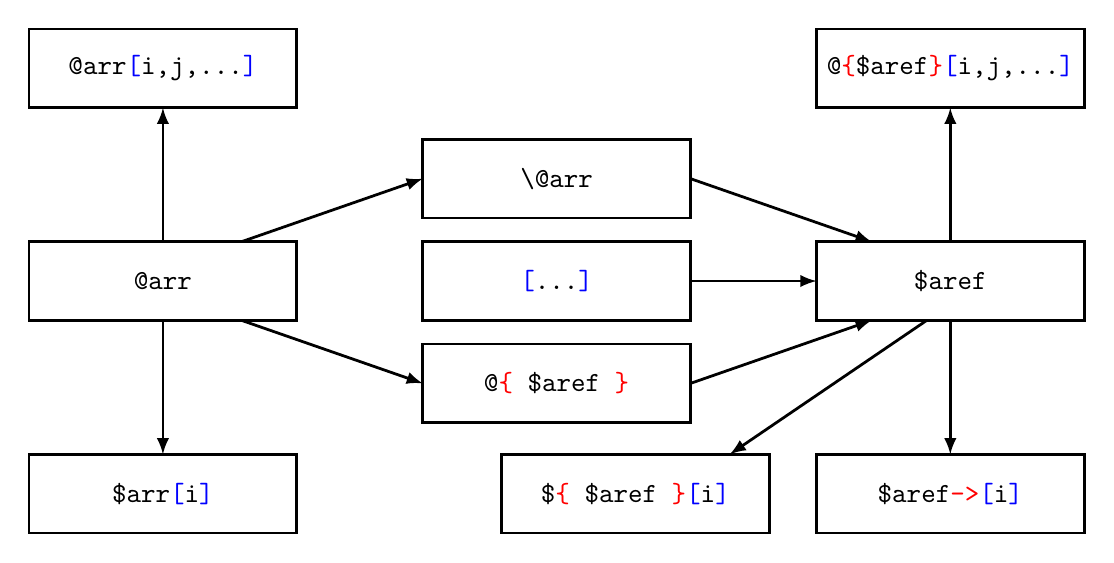
\begin{tikzpicture}[line width=1pt] \def\setpoints#1(#2)#3<#4,#5>#6 at (#7);{
		\path[shift={(#7)}]
		( 0     , 0      ) coordinate (#2)
		( 0.5*#4, 0      ) coordinate (#2_east)
		( 0     , 0.5*#5 ) coordinate (#2_north)
		(-0.5*#4, 0      ) coordinate (#2_west)
		( 0     ,-0.5*#5 ) coordinate (#2_south)
		( 0.5*#4, 0.5*#5 ) coordinate (#2_north_east)
		(-0.5*#4, 0.5*#5 ) coordinate (#2_north_west)
		( 0.5*#4,-0.5*#5 ) coordinate (#2_south_east)
		(-0.5*#4,-0.5*#5 ) coordinate (#2_south_west); }



\def\doit{\draw[latex-] (box_west) -- (s); \draw[-latex] (box_east) -- (e);}
\def\stepbl{\path (current)+(0,-7mm) coordinate (current);}
\def\dblock<#1>(#2){
		\setpoints (box) <30mm,6mm> at (current);
		\draw[fill={#1}] (box_south_west) rectangle (box_north_east) (box) node {#2};
		\doit\stepbl }
\def\dblockl<#1>(#2){
		\setpoints (box) <30mm,6mm> at (current);
		\setpoints (box_in)  <6mm,6mm> at ($(box_west)+(0.3,0)$);
		\draw[fill={#1}] (box_in_south_west) rectangle (box_in_north_east) (box_in) node {$\wedge$};
		\draw[-latex] (box_in_east) --+ (4mm,0);
		\setpoints (box_in)  <20mm,6mm> at ($(box_west)+(2,0)$);
		\draw[fill={#1}] (box_in_south_west) rectangle (box_in_north_east) (box_in) node {#2};
		\doit\stepbl }
\def\dsmallblock<#1><#2> (#3) at (#4);{ \setpoints (box) <#1> at (#4);
		\draw[fill={#2}] (box_south_west) rectangle (box_north_east);
		\draw (box) node {#3}; }
	
	\def\block#1(#2)#3<#4>[#5] at (#6);{
		\setpoints (#2) <#4> at (#6);
		\draw (#2_south_west) rectangle (#2_north_east) (#2) node {\texttt{#5}};
	}
	
	
%---------------------------------------------

\def\block#1(#2)#3<#4>[#5] at (#6);{
	\setpoints (#2) <#4> at (#6);
	\draw (#2_south_west) rectangle (#2_north_east) (#2) node {\texttt{#5}};
}
\def\arr<#1>{\textcolor{blue}{[}#1\textcolor{blue}{]}}
\def\h<#1>{\textcolor{blue}{\{}#1\textcolor{blue}{\}}}
\def\curv<#1>{\textcolor{red}{\{}#1\textcolor{red}{\}}}
\def\red|#1|{\textcolor{red}{#1}}	
\block (c) <3.4cm,1cm>[@arr] at (0, 0);
\block (u) <3.4cm,1cm>[@arr\arr<i,j,...>] at (0, 2.7);
\block (d) <3.4cm,1cm>[\$arr\arr<i>]       at (0,-2.7);
\draw[-latex] (c_north) -- (u_south);
\draw[-latex] (c_south) -- (d_north);

\block (u) <3.4cm,1cm>[\textbackslash@arr] at (5, 1.3);
\block (d) <3.4cm,1cm>[@\curv<\ \$aref >]       at (5,-1.3);
\draw[-latex] (c_north)+(1,0) -- (u_west);
\draw[-latex] (c_south)+(1,0) -- (d_west);
\block (c) <3.4cm,1cm>[\$aref]       at (10,0);
\draw[latex-] (c_north)+(-1,0) -- (u_east);
\draw[latex-] (c_south)+(-1,0) -- (d_east);

\block (ct) <3.4cm,1cm>[\arr<...>] at (5, 0);
\draw[latex-] (c_west) -- (ct_east);

\block (u) <3.4cm,1cm>[@\curv<\$aref>\arr<i,j,...>]       at (10,2.7);
\block (d) <3.4cm,1cm>[\$aref\red|->|\arr<i>]       at (10,-2.7);

\draw[-latex] (c_north) -- (u_south);
\draw[-latex] (c_south) -- (d_north);

\block (d) <3.4cm,1cm>[\$\curv<\ \$aref >\arr<i>]       at (6,-2.7);
\draw[-latex] (c_south)+(-0.3,0) -- ($(d_north_east)+(-0.5,0)$);

\end{tikzpicture}
	\caption{Способы записи ссылок на массивы}
\end{figure}

Обычный массив записывается в виде <<$@$ плюс идентификатор>>.
Если нужно взять на него ссылку, то добавляется~$\backslash$ и получается скалярная переменная, в которой находится ссылка на исходный массив (см.~рис.~3).
Можно также сделать анонимный конструктор.

Если же из ссылки нужно получить массив с~$@$, то есть передать какую-либо функцию или просто развернуть список, то производится операция разыменования ($@\{\}$).
Фигурные скобки иногда можно опустить (в случае, если это очевидно).
Разыменование является обратным преобразованием.

В следующем примере используется оператор \textit{qw}, разделяющий свое содержимое по пробельным символам:

%00:20:29
\pr<code/L01_code_023.pl>

Необходимо отметить, что массив всегда инициализируется списком.

У массивов есть \textit{срезы}, используемые для того, чтобы достать из массива часть в виде списка.
Здесь используется специальный синтаксис, который встречается довольно редко: идентификатор вместе с квадратными скобками записывается внутри фигурных скобок:

%00:22:37
\pr<code/L01_code_024.pl>

Аналогично для ссылок~--- на то место, где был идентификатор переменной, подставляется ссылка.
Так как идентификатор сам по себе является переменной, то и к нему можно добавить фигурные скобки:

%00:22:37
\pr<code/L01_code_025.pl>

Везде, где у массивов квадратные скобки, у хэшей фигурные.
Хэш определяется с помощью знака~$\%$, ссылка берется так же, как и у массивов, разыменование берется процентом (см.~рис.~4).
Хэш конструируется анонимно при помощи фигурных скобок.
Обращение к одному элементу~--- фигурные скобки плюс ключ, обращение скалярное.

%Рис. 4: 00:22:37
\begin{figure}[h!]\center
	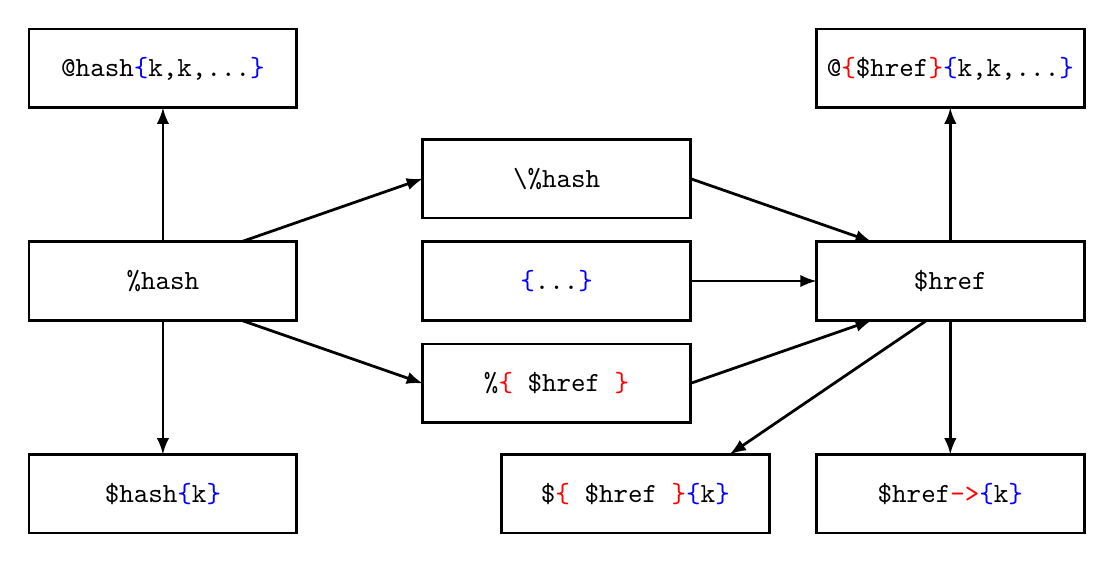
\begin{tikzpicture}[line width=1pt] \def\setpoints#1(#2)#3<#4,#5>#6 at (#7);{
		\path[shift={(#7)}]
		( 0     , 0      ) coordinate (#2)
		( 0.5*#4, 0      ) coordinate (#2_east)
		( 0     , 0.5*#5 ) coordinate (#2_north)
		(-0.5*#4, 0      ) coordinate (#2_west)
		( 0     ,-0.5*#5 ) coordinate (#2_south)
		( 0.5*#4, 0.5*#5 ) coordinate (#2_north_east)
		(-0.5*#4, 0.5*#5 ) coordinate (#2_north_west)
		( 0.5*#4,-0.5*#5 ) coordinate (#2_south_east)
		(-0.5*#4,-0.5*#5 ) coordinate (#2_south_west); }



\def\doit{\draw[latex-] (box_west) -- (s); \draw[-latex] (box_east) -- (e);}
\def\stepbl{\path (current)+(0,-7mm) coordinate (current);}
\def\dblock<#1>(#2){
		\setpoints (box) <30mm,6mm> at (current);
		\draw[fill={#1}] (box_south_west) rectangle (box_north_east) (box) node {#2};
		\doit\stepbl }
\def\dblockl<#1>(#2){
		\setpoints (box) <30mm,6mm> at (current);
		\setpoints (box_in)  <6mm,6mm> at ($(box_west)+(0.3,0)$);
		\draw[fill={#1}] (box_in_south_west) rectangle (box_in_north_east) (box_in) node {$\wedge$};
		\draw[-latex] (box_in_east) --+ (4mm,0);
		\setpoints (box_in)  <20mm,6mm> at ($(box_west)+(2,0)$);
		\draw[fill={#1}] (box_in_south_west) rectangle (box_in_north_east) (box_in) node {#2};
		\doit\stepbl }
\def\dsmallblock<#1><#2> (#3) at (#4);{ \setpoints (box) <#1> at (#4);
		\draw[fill={#2}] (box_south_west) rectangle (box_north_east);
		\draw (box) node {#3}; }
	
	\def\block#1(#2)#3<#4>[#5] at (#6);{
		\setpoints (#2) <#4> at (#6);
		\draw (#2_south_west) rectangle (#2_north_east) (#2) node {\texttt{#5}};
	}
	
	
%---------------------------------------------

\def\block#1(#2)#3<#4>[#5] at (#6);{
	\setpoints (#2) <#4> at (#6);
	\draw (#2_south_west) rectangle (#2_north_east) (#2) node {\texttt{#5}};
}
\def\arr<#1>{\textcolor{blue}{[}#1\textcolor{blue}{]}}
\def\h<#1>{\textcolor{blue}{\{}#1\textcolor{blue}{\}}}
\def\curv<#1>{\textcolor{red}{\{}#1\textcolor{red}{\}}}
\def\red|#1|{\textcolor{red}{#1}}	
\block (c) <3.4cm,1cm>[\%hash] at (0, 0);
\block (u) <3.4cm,1cm>[@hash\h<k,k,...>] at (0, 2.7);
\block (d) <3.4cm,1cm>[\$hash\h<k>]       at (0,-2.7);
\draw[-latex] (c_north) -- (u_south);
\draw[-latex] (c_south) -- (d_north);

\block (u) <3.4cm,1cm>[\textbackslash\%hash] at (5, 1.3);
\block (d) <3.4cm,1cm>[\%\curv<\ \$href >]       at (5,-1.3);
\draw[-latex] (c_north)+(1,0) -- (u_west);
\draw[-latex] (c_south)+(1,0) -- (d_west);
\block (c) <3.4cm,1cm>[\$href]       at (10,0);
\draw[latex-] (c_north)+(-1,0) -- (u_east);
\draw[latex-] (c_south)+(-1,0) -- (d_east);

\block (ct) <3.4cm,1cm>[\h<...>] at (5, 0);
\draw[latex-] (c_west) -- (ct_east);

\block (u) <3.4cm,1cm>[@\curv<\$href>\h<k,k,...>]       at (10,2.7);
\block (d) <3.4cm,1cm>[\$href\red|->|\h<k>]       at (10,-2.7);

\draw[-latex] (c_north) -- (u_south);
\draw[-latex] (c_south) -- (d_north);

\block (d) <3.4cm,1cm>[\$\curv<\ \$href >\h<k>]       at (6,-2.7);
\draw[-latex] (c_south)+(-0.3,0) -- ($(d_north_east)+(-0.5,0)$);

\end{tikzpicture}
	\caption{Способы записи ссылок на хэши}
\end{figure}

У хэша тоже есть срез.
Так как срез является списковым обращением, то используется~$@$, а не~$\%$ (см.~рис.~4).
Обращение к ссылке происходит подобным образом (разыменование ссылки, обращение к фигурным скобкам, перечисление ключей).

Из следующего примера видно, что хэш конструируется так же, как и массив (списком).
В качестве указания ключа можно использовать внутри фигурных скобок \textit{Bareword} (можно без кавычек):

%00:25:08
\pr<code/L01_code_026.pl>

Сложный ключ можно взять в любые кавычки.
В качестве ключа можно использовать переменную.

Аналогичный пример для срезов:

%00:26:46
\pr<code/L01_code_027.pl>

В отличие от массива, хэш можно развернуть в список.
Важная особенность Perl: хэши являются несортированными, то есть неважно, в каком порядке их исходно присваивали.
Есть специальные функции \textit{keys} и \textit{values}, которые возвращают соответственно ключи хэша и значения, им соответствующие.
При этом порядок, который вернет \textit{keys}, и порядок, который вернет \textit{values}, будет одинаковым.
В ключ хэша можно присваивать значения или удалять значения из него.
<<Жирная>> запятая ($\Rightarrow$) влияет на свой левый операнд: если он является \textit{Bareword}, то вокруг него ставятся кавычки.

С помощью ссылок можно создавать сложные структуры.
Если присваивается хэш или массив, то используются круглые скобки.
При инициализации элементы не должны быть одного типа.
Можно заметить, что зачастую <<жирная>> запятая используется, даже если это не требуется левому операнду.
В отличие от обычного хэша, который конструируется списком, ссылка на хэш конструируется фигурными скобками:

%00:28:59
\pr<code/L01_code_028.pl>

Самая частая проблема у того, кто только начинает писать на Perl~--- путаница между массивами и ссылками на массив.
Если в следующем примере создать массив и положить в него вместо круглых скобок квадратные, то получится массив, единственным элементом которого будет ссылка на массив:

%00:31:28
\pr<code/L01_code_029.pl>

Аналогичная проблема возникает с хэшем:

%00:31:28
\pr<code/L01_code_030.pl>

Другая проблема часто возникает при сборке хэша: вместо массива используется список.
В данном примере в итоге получится список из шести элементов, которые попарно будут обращены в хэш:

%00:31:28
\pr<code/L01_code_031.pl>

Таким образом, если что-то идет не так, в первую очередь необходимо обратить внимание на то, как именно конструируются структуры.

В случае хэша или массива можно обращаться к несуществующим элементам.
При этом Perl по пути будет создавать недостающие элементы, если обращаться к ним глубже:

%00:33:06
\pr<code/L01_code_032.pl>

Если в данном примере обратиться к существующему элементу, который не является ссылкой, то логично, что программа должна <<упасть>>, однако, этого не происходит.
Более того, в процессе создается хэш с именем \textit{string}.

Это явление носит название \textit{символическая ссылка} (переменная, чьё значение является именем другой переменной).
Так как язык является динамическим, переменные могут создаваться <<на лету>> (их не обязательно объявлять заранее), а также можно обратиться к переменной, чье имя известно из другой переменной.
В следующем примере к переменной обращаются как к ссылке, как к массиву и как к хэшу:

%00:35:11
\pr<code/L01_code_033.pl>

Хоть символические ссылки бывают удобны при создании <<однострочных>> программ, их использование являются плохим подходом в программах более сложного уровня.
В связи с этим полезен модуль \textit{strict}, параметр \textit{refs} которого запрещает использование символических ссылок:

%00:36:39
\pr<code/L01_code_034.pl>

Важно заметить, что если внутри фигурных скобок записан \textit{Bareword}, то это не является символической ссылкой.
Когда в хэш передается \textit{Bareword}, он его автоматически заключает в кавычки.
Есть некоторые встроенные функции, которые можно явно называть, например, функция \textit{shift}.
Если нужно явно сказать, что внутри фигурных скобок стоит \textit{expression}, то можно либо добавить унарный оператор~$+$, либо вызвать функцию со скобками.

\subsection{Интерполяция}
Внутри двойных кавычек интерполируются переменные, то есть можно непосредственно в строке использовать значение другой переменной.
В строках интерполируются~$\$\dots$ и~$@\dots$.
Внутри кавычек также можно использовать списковый контекст ($\$$), срезы и хэши:

%00:39:14
\pr<code/L01_code_035.pl>

Здесь~$\S''$~--- это \textit{list separator}, разделитель.

Так как в интерполяции используются~$\$$ или~$@$, при этом~$\$\{\}$ или~$@\{\}$являются операторами разыменования ссылки, а внутри фигурных скобок можно использовать любой \textit{expression}, то можно писать какой-либо исполняемый код внутри ссылок:

%00:41:41
\pr<code/L01_code_036.pl>

Из примера видно, что здесь возможно использовать не только списочный конструктор, но и скалярный.

\renewcommand{\lasttiming}{2625}
\section{Функции} %00:43:45:00 - Функции (декларация, аргументы, контекст, прототипы, встроенные функции, grep, map, sort, eval)

\subsection{Декларация, аргументы}
\textit{Функции} в общем виде записываются следующим образом:

%00:44:09
\pr<code/L01_code_037.pl>

Можно заранее продекларировать функцию с определенным именем или с некоторым прототипом (без тела).
Анонимные функции конструируются без объявления имени:

%00:44:09
\pr<code/L01_code_038.pl>

Такие функции всегда возвращают свое значение, и его можно присвоить в какую-либо переменную.

Пример объявления функции:

%00:44:50
\pr<code/L01_code_039.pl>

Все аргументы функции размещаются в спецпеременной~$@\_$.
Функции работы с массивами по умолчанию работают с таким массивом.
В примере также показаны две наиболее часто используемые формы взятия аргументов функции.
Если пишется компактная функция, которая должна быстро работать (например, она часто используется в программе), то можно обратиться к конкретному элементу из аргументов напрямую.

\subsection{Контекст}
Функции <<чувствуют>> контекст, в котором их вызывают.
Для вызова функции существует три контекста.
\textit{Скалярный контекст} означает, что результат функции присваивается в скалярную переменную (либо с функцией выполняется какое-то скалярное действие):

%00:46:34
\pr<code/L01_code_040.pl>

В \textit{списковом контексте} результат функции либо помещается в массив, либо присваивается какому-то списку:

%00:46:34
\pr<code/L01_code_041.pl>

\textit{Void-контекст} означает, что функция просто вызывается, а её результат не представляет интереса:

%00:46:34
\pr<code/L01_code_042.pl>

Контекст проверяется при помощи специального вызова \textit{wantarray}:

%00:47:08
\pr<code/L01_code_043.pl>

При void-вызове \textit{wantarray} будет \textit{undefined}.
Если контекст списковый, то \textit{wantarray} будет \textit{true}, если скалярный~--- \textit{false}.

В теле функции можно написать \textit{return}.
Можно сделать \textit{return} без каких-либо результатов, можно вернуть один элемент, можно вернуть список.
Любой последний \textit{statement} в теле функции является автоматически возвращаемым значением.

Самый простой способ вызова функции~--- дописать к ней круглые скобки и передать аргументы:

%00:48:13
\pr<code/L01_code_044.pl>

Если функция была объявлена раньше, то круглые скобки можно опустить.
Существует <<старый>> стиль записи~--- с использованием~$\&$ и круглых скобок:

%00:48:13
\pr<code/L01_code_045.pl>

Такой синтаксис вызова применялся в Perl четвертой версии.
Самостоятельно использовать данный стиль записи не рекомендуется.
Вызов функции с текущими аргументами имеет вид:

%00:48:13
\pr<code/L01_code_046.pl>

Вызвать ссылку на функцию можно несколькими способами:

%00:48:13
\pr<code/L01_code_047.pl>

\subsection{Прототипы}
У функции может быть объявлен \textit{прототип} (перечисление того, что функция хочет на вход).
Например, можно объявить, что функция принимает ровно два аргумента, и тогда при попытке вызвать её с другим количеством аргументов программа не скомпилируется.
Можно также сказать, что функция хочет первым аргументом скаляр, список, файловый дескриптор, указатель на функцию или разделитель:

%00:50:08
\pr<code/L01_code_048.pl>

Существуют и более расширенные прототипы:

%00:50:08
\pr<code/L01_code_049.pl>

Если прототип пустой, то функция не принимает никаких аргументов.

Специальный прототип~$\&$, находясь в первой позиции, позволяет употреблять подобный синтаксис:

%00:52:15
\pr<code/L01_code_050.pl>

В данном случае функция таким образом проверяет, что все аргументы на вход меньше десяти.

\subsection{Встроенные функции:grep, map, sort}
Есть встроенные функции, которые ведут себя подобным образом~--- \textit{grep}, \textit{map} и \textit{sort}.

Функция \textit{grep} принимает на вход список, для каждого элемента которого устанавливает значение в~$\$\_$ и вызывает переданный блок.
Блок должен вернуть \textit{true} или \textit{false}.
Если блок возвращает \textit{true}, элемент пропускается в выход.
Таким образом, данная функция является своеобразным фильтром:

%00:53:22
\pr<code/L01_code_051.pl>

Здесь представлен также упрощенный синтаксис \textit{grep}, работающий без фигурных скобок.

Функция \textit{map} позволяет взять входной список и преобразовать его в какой-то другой список.
Для каждого элемента списка \textit{map} вызывает блок, а то, что возвращает блок, помещается в исходящий список.
Данная функция тоже может принимать не обязательно блок, можно написать вместо него \textit{expression}:

%00:54:29
\pr<code/L01_code_052.pl>

Функция \textit{map} может вернуть пустой список (\textit{map} может быть использован как частный случай \textit{grep}).

Функция \textit{sort} сортирует входящий список:

%00:55:19
\pr<code/L01_code_053.pl>

Синтаксически \textit{sort} может либо просто принять список (тогда отсортирует лексикографически), либо принять блок компаратора, либо принять имя функции, в которой реализован компаратор.
Компаратор должен вернуть одно из трех значений:~$-1,0,1$.
В зависимости от этого сортируется исходящий список.

В языке Perl есть некоторое количество функций, которые ведут себя по-разному в зависимости от того, какие аргументы им передаются.
Одной из таких функций является \textit{eval}.
Пример простейшего \textit{try-catch}:

%00:56:50
\pr<code/L01_code_054.pl>

С обычным скалярным аргументом функция \textit{eval} берет то, что написано в этом аргументе, и исполняет это как код Perl.
Если у \textit{eval} не получится выполнить этот код, то он установит специальную переменную~$\$@$ с текстом ошибки.

Возможен блочный вызов для функции \textit{eval}.
Внутри него находится код, уже прошедший синтаксическую проверку, то есть происходит перехват исключений.
Исключения можно выбросить при помощи ключевого слова \textit{die}.
За написание предупреждений отвечает \textit{warn} (пишет, в какой строке произошло).

Важными встроенными функциями являются \textit{chop} и \textit{chomp}.
Функция \textit{chop} отрубает с конца один символ, а функция \textit{chomp} отрезает с конца строки то, что содержится в разделителе входного потока:

%00:59:00
\pr<code/L01_code_055.pl>

Для работы со строками есть стандартный набор из Си (\textit{index}, \textit{rindex}, \textit{substr}, \textit{lenght}):

%00:59:00
\pr<code/L01_code_055_2.pl>

Существуют также функции приведения кейса \textit{lc}, \textit{lcfirst}, \textit{uc}, \textit{ucfirst}, \textit{fc}:

%00:59:33
\pr<code/L01_code_056.pl>

Функции \textit{chr}, \textit{ord}, \textit{hex}, \textit{oct} используются для преобразования символа в код и кода в символ:

%01:01:33
\pr<code/L01_code_057.pl>

Функция \textit{reverse} имеет двойное поведение.
В скалярном контексте \textit{reverse} переворачивает тот скаляр, который ему дали, а в списковом контексте он переворачивает список целиком, не изменяя его элементы.
На эту тему имеется шутка:

%01:01:55
\pr<code/L01_code_058.pl>

Примеры разных форматов для функции \textit{sprintf}, знакомые многим по Си:

%01:01:55
\pr<code/L01_code_059.pl>

\subsection{eval}
В языке Perl есть многие необходимые математические функции (\textit{abs}, \textit{int}, \textit{srand}, \textit{rand}, \textit{log}, \textit{exp}, \textit{sin}, \textit{cos}, \textit{atan2}, \textit{sqrt}).
Они ведут себя практически так же, как и соответствующие операторы из Си.
Следующий пример показывает, почему нужно смотреть на класс точности \textit{double}:

%01:01:55
\pr<code/L01_code_060.pl>

Для работы с хэшами используются функции \textit{keys}, \textit{values} и итератор \textit{each}:

%01:04:11
\pr<code/L01_code_061.pl>
\begin{comment}
0: 1 (-1)
1: 3 (-3)
2: 2 (-2)
1: -1
3: -3
2: -2
\end{comment}

Итератор \textit{each} последовательно возвращает попарно элементы данного хэша или массива.
Это способ обойти весь массив или хэш.

Для работы с массивами используются функции \textit{push}, \textit{pop}, \textit{shift}, \textit{unshift}, \textit{splice}:

%01:04:35
\begin{table}[H] \centering
\begin{tabular}{ll} \hline\hline
push(@a,\$x,\$y)    & splice(@a,@a,0,\$x,\$y) \\
pop(@a)             & splice(@a,-1)\\
shift(@a)           & splice(@a,0,1)\\
unshift(@a,\$x,\$y) & splice(@a,0,0,\$x,\$y)\\
\$a[\$i] = \$y      & splice(@a,\$i,1,\$y)\\
\hline\hline
\end{tabular}
\end{table}

По умолчанию все эти функции работают с массивом аргументов функции~$@\_$.
Функция \textit{splice} позволяет любым образом нарезать массив:

%01:04:35
\pr<code/L01_code_061_2.pl>


Для работы со временем есть функции \textit{gmtime}, \textit{localtime}, \textit{time} и \textit{strftime}:

%01:05:39
\pr<code/L01_code_062.pl>

Perl обладает стеком, для работы с которым используются функции \textit{caller} и \textit{goto}:

%01:06:29
\pr<code/L01_code_063.pl>

При работе с функциями при необходимости следует изучать документацию, не обязательно помнить все особенности функций наизусть.

\renewcommand{\lasttiming}{4616}
\section{Операторы} %01:07:56:00 - Операторы (порядок использования, особенные операторы, числа и строки)
\subsection{Порядок исполнения}
В отличие от большинства динамических языков, Perl смотрит не на тип операнда, а на тип оператора.
В Perl есть отдельно числовые операторы и строковые.
Если на вход числового оператора приходят строки, они будут преобразованы в числа (и наоборот).
Ассоциативность и приоритет арифметических операторов соответствуют тому, как это принято в математике.

Здесь перечислены все операторы, которые есть в языке Perl:

%01:09:06

\begin{table}[H] \centering
\def\o(#1){\colorbox{gray!20}{\texttt{#1}\phantom{/}\!\!\!\!}}
\begin{tabular}{|c|c|} \hline
Ассоциативность & Оператор \\ \hline
left&	TERM и LIST \\ \hline
left&	\o(->) \\ \hline
n/a&	\o(++), \o(-\textrm{-}) \\ \hline
right&	\o(**) \\ \hline
right&	\o(!), \o($\sim$), \o(\textbackslash) unary \o(+), \o(-), \\ \hline
left&	\o(=~) \o(!~) \\ \hline
left&	\o(*), \o(/), \o(\%), \o(\times) \\ \hline
left&	\o(+), \o(-), \o(.)\\ \hline
left&	\o(<<), \o(>>)\\ \hline
n/a&	named unary ops\\ \hline
n/a&	\o(<),\o(>),\o(<=),\o(>=), \o(lt), \o(gt), \o(le), \o(ge)\\ \hline
n/a&	\o(==), \o(!=), \o(<=>), \o(eq), \o(ne), \o(cmp), \o($\sim$$\sim$)\\ \hline
... & ... \\ \hline
\end{tabular}
\begin{tabular}{|c|c|} \hline
Ассоциативность & Оператор \\ \hline
... & ... \\ \hline
left&	\o(\&) \\ \hline
left&	\o(|), \o($\wedge$) \\ \hline
left&	\o(\&\&) \\ \hline
left&	\o(||), \o(//) \\ \hline
n/a&	\o(..), \o(...)\\ \hline
right&	\o(?:) \\ \hline
right&	\o(=), \o(+=), \o(-=), \o(*=) и т.д.\\ \hline
left&	\o(,), \o(=>)\\ \hline
n/a&	LIST\\ \hline
right&	\o(not)\\ \hline
left&	\o(and)\\ \hline
left&	\o(or), \o(xor)\\ \hline
\end{tabular}
\end{table}


Операторы перечислены в порядке приоритета и с указанием ассоциативности.

\subsection{Операторы TERM и LIST}
Самыми высокоприоритетными оператором являются \textit{TERM} и \textit{LIST (L)}:

%01:09:43
\begin{comment}
Любая переменная ($variable)
Обращение к хэшу или массиву ($hash{key} или $array[$x])
Любая строка ("string" или 'str'), число (42, -1e42) или quote-
like оператор
Любой вызов функции со скобками func(...)
do{ ... }, eval{ ... }, sub{ ... }
Анонимные конструкторы
{ ... } и [ ... ]
\end{comment}

Чтобы понять, как именно Perl разбирается с таким количеством операторов, можно рассмотреть следующий пример:

%01:11:00
\pr<code/L01_code_064.pl>

С первого взгляда непонятно, в какой последовательности будут выполнены действия.
Бывает уместно воспользоваться модулем \textit{Deparse}~--- он расставит скобки:

%01:11:00
\pr<code/L01_code_065.pl>

Можно рассмотреть действия по шагам:

%01:11:44
\pr<code/L01_code_066.pl>

\subsection{Оператор <<стрелочка>>}
Следующий оператор по приоритету~--- <<стрелочка>> ($\to$, \textbf{суффиксный оператор разыменования}).
Зачастую он относится к идентификатору переменной.
У него есть еще два вызова: вызов метода на объекте или классе и вызов метода по содержимому переменной:

%01:13:19
\pr<code/L01_code_067.pl>

\subsection{Операторы инкремента и декремента}
Далее по приоритету~--- \textbf{операторы инкремента} и \textbf{декремента} (аналогичны соответствующим в Си):

%01:13:36
\pr<code/L01_code_068.pl>

Здесь нужно отметить, что~$++\$i + \$i++$ является неопределённым поведением.
Если в качестве аргумента этим операторам передается \textit{undef}, то он всегда работает как число 0.

В языке Perl оператор~$++$ наделен <<магическим>> поведением.
Данный оператор работает не только над числами, но и над строками.
Если переменная, попадающая в оператор инкремента, является строкой, начинается на большие или маленькие буквы и содержит в себе буквы или цифры, то она используется как число, знаковым набором которого являются соответствующие диапазоны:

%01:14:56
\pr<code/L01_code_069.pl>

При этом декремент <<магическим>> не является.

\subsection{Унарные операторы}
В Perl существует привычный по Си \textbf{оператор логического отрицания} ($!$).
В данном языке \textit{false}~--- это~$0$, пустая строка, \textit{undef} и \textit{overloaded object}.
\textit{True}~--- все остальное, по умолчанию~$1$:

%01:16:28
\pr<code/L01_code_070.pl>

Унарный оператор~$-$ (\textbf{математическое отрицание}) на числах меняет знак числа.
В Perl у него также определено поведение на строках и на \textit{Bareword}:

%01:16:53
\pr<code/L01_code_071.pl>

Унарный \textbf{оператор битовой инверсии} ($\sim$) работает как на числах, так и на строках, демонстрируя двойственное поведение:

%01:18:33
\pr<code/L01_code_072.pl>

Унарный оператор~$+$ не имеет собственного эффекта и используется как разделитель, когда нужно понизить приоритет:

%01:19:26
\pr<code/L01_code_073.pl>

Иногда~$+$ используется как обозначение, что далее следует конструктор анонимного хэша:

%01:19:26
\pr<code/L01_code_074.pl>

В языке Perl есть оператор, редко встречающийся в других языках~--- \textbf{оператор применения регулярного выражения}, позитивный и негативный ($=\sim$,~$!\sim$):

%01:21:44
\pr<code/L01_code_075.pl>

Необходимо заметить, что пробел между~$=$ и~$\sim$ не должен ставиться, иначе один оператор превратится в два.

\subsection{Числа и строки}
Существуют также привычные \textbf{операторы арифметики} ($^{\ast}$,~$/$,~$\%$).
Они работают на числах и приводят все к числам:

%01:22:25
\pr<code/L01_code_076.pl>

Нестандартный оператор~$\times$~--- это \textbf{оператор повтора}, работающий либо на скалярах, либо на списках:

%01:22:25
\pr<code/L01_code_077.pl>

\textbf{Бинарные операторы} сложения, вычитания и конкатенации ($+$,~$-$,~$.$) работают следующим образом:

%01:23:01
\pr<code/L01_code_078.pl>

Необходимо быть аккуратнее при использовании конкатенации~--- если слева и справа от точки стоят числа, то это число с десятичной частью, в случае конкатенации нужно отделять числа от точки пробелами.

\textbf{Оператор сдвига} ($\ll$,~$gg$) реализован полностью с использованием Си, и его поведение аналогично:

%01:23:01
\pr<code/L01_code_079.pl>

\textbf{Операторы сравнения} разделены на арифметические ($<$,~$>$,~$<=$,~$>=$) и строковые (\textit{lt}, \textit{gt}, \textit{le}, \textit{ge}):

%01:24:25
\pr<code/L01_code_080.pl>

Аналогично \textbf{операторы равенства}~$==$,~$!=$ и~$<=>$ работают исключительно с числами, а строковые операторы \textit{eq}, \textit{ne}, \textit{cmp} работают только со строками:

%01:25:23
\pr<code/L01_code_081.pl>

Так как изначально в язык не заложено таких понятий как \textit{NaN}, они здесь реализованы строками.
Понять, поддерживается ли данная платформа, можно следующим образом:

%01:25:23
\pr<code/L01_code_082.pl>

В Perl версии~$5.10.1$ внердили \textit{smartmatch operator}~--- \textbf{оператор умного сравнения} ($\sim\sim$).
Этот оператор <<вшит>> в \textit{given/when}, но его можно использовать и вручную:

%01:26:45
\pr<code/L01_code_083.pl>

Однако, этот оператор оказался настолько сложным в использовании, что в Perl версии~$5.18$ и выше его снова признали экспериментальным.


\textbf{Битовые операторы} \textit{and}, \textit{or} и \textit{xor} ($\&$,~$|$,~$\^$) работают раздельно над числами и над строками:

%01:27:59
\pr<code/L01_code_084.pl>

Если операнды смешанные, то берется тип левого операнда, и второй приводится к нему.

Существуют также \textbf{C-style логические операторы} \textit{and}, \textit{or}, \textit{defined-or} ($\&\&$,~$||$,~$//$).
Они выполняются последовательно и передают контекст:

%01:30:00
\pr<code/L01_code_085.pl>

Оператор \textit{defined-or} находится в данной категории по смыслу, но у него нет аналогов в других языках.
Данный оператор проверяет переменную не на <<\textit{true/false}>>, а на то, что она \textit{defined}.
У этих операторов очень высокий приоритет по сравнению с обычным списком, в связи с этим могут возникать определенные трудности.

\subsection{Операторы диапазона}
В Perl есть \textbf{операторы диапазона}, \textit{range operators} ($..$,~$\dots$).
Эти операторы работают по-разному в разных контекстах.
В списковом контексте они просто возвращают соответствующий список, как показано в следующем примере:

%01:31:31
\pr<code/L01_code_086.pl>


Если же оператор диапазона применен в скалярном (логическом) контексте, то он проверяет переменную~$\$.$ на соответствие граничным значениям.
Пример с константным операндом:

%01:32:15
\pr<code/L01_code_087.pl>


В качестве операнда в данном контексте может быть использовано выражение:

%01:34:38
\pr<code/L01_code_088.pl>

Можно расписать действия оператора по шагам:

%01:35:40
\pr<code/L01_code_089.pl>

Отличия между оператором~$..$ и оператором~$\dots$ состоит в том, что на втором шаге (когда становится истинным левое выражение) второй оператор не пытается проверять правое выражение.
В основном операторы диапазона используются в списковом контексте.

\subsection{Тернарный оператор}
\textbf{Тернарный оператор} ($?:$) в Perl аналогичен оператору из Си (за исключением того, что в него можно присваивать):

%01:37:32
\pr<code/L01_code_090.pl>

\subsection{Операторы присваивания}
\textbf{Операторы присваивания} работают относительно всех операторов, которые есть в языке Perl:

%01:37:44
\begin{itemize}[nosep]
\item += -=
\item *= /= \%= **=
\item \&= |= x= <<= >>= $\wedge$=
\item \&\&= ||= //=
\end{itemize}

Данные операторы того же приоритета, что и~$=$ (не разбиваются по приоритетам относительно исходных операторов).

\subsection{Оператор запятая}
\textbf{Оператор запятая} делится на обычную и <<жирную>> ($,$,~$\Rightarrow$).
За исключением работы с \textit{Bareword}, эти операторы работает одинаково:

%01:38:16
\pr<code/L01_code_091.pl>

В скалярном контексте данный оператор исполняет свой левый операнд, затем выбрасывает это значение, исполняет правый и возвращает его значение.
В списковом контексте этот оператор возвращает тот список, который получается.

В Perl функция с пустым прототипом и с константным значением является константой.
Если написать константу слева от <<жирной>> запятой, то она сделает из константы строку, что является важной особенностью этого оператора:

%01:38:16
\pr<code/L01_code_092.pl>

\subsection{Низкоприоритетные логические операторы}
\textbf{Низкоприоритетные логические операторы} \textit{and}, \textit{or}, \textit{xor} и \textit{not} являются операторами с самым низким приоритетом из возможных:

%01:40:50
\pr<code/L01_code_093.pl>

Такие операторы используются, например, для проверки возвращаемого значения функций.

\subsection{Оператор кавычки}
\textbf{Оператор кавычки}~--- \textit{q}, \textit{qq}, \textit{qw}, \textit{qx}, \textit{qr}, \textit{s}, \textit{y}, \textit{tr}, довольно однотипные.
Оператор \textit{q}~--- это строка без интерполяции:

%01:43:55
\pr<code/L01_code_094.pl>

По сути~$q$ аналогичен одинарным кавычкам.
Здесь разделителем может быть любой символ (в примере~--- \textit{q}), кроме пробельного символа.

Оператор \textit{qq}~--- строка с интерполяцией (двойные кавычки):

%01:45:55
\pr<code/L01_code_095.pl>

Оператор \textit{qw}~--- генератор списка (без интерполяции):

%01:46:07
\pr<code/L01_code_096.pl>

Все, что записано внутри оператора \textit{qw} и разделено по пробельным символам, будет возвращено в виде одного списка.
Данный оператор часто используется при вызове внешних модулей.
В качестве разделителя снова может использоваться любой символ, чаще всего используются~$/$ либо круглые скобки.

Оператор \textit{qx} позволяет выполнить внешнюю команду (обратные кавычки):

%01:47:20
\pr<code/L01_code_097.pl>

Данный оператор является интерполируемым, но если в качестве разделителя поставить одинарные кавычки, то он перестанет быть таковым.

Оператор \textit{qr}~--- сборка регулярного выражения:

%01:47:58
\pr<code/L01_code_098.pl>

Здесь~$/\dots/$ или \textit{m}~--- это сопоставление (\textit{match}), \textit{s}~--- поиск и замена (\textit{replace}), \textit{y} или \textit{tr}~--- транслитерация.

Помимо оператора кавычек для сборки строк существует \textit{Here-doc} (угловые скобки с последующим идентификатором):

%01:49:15
\pr<code/L01_code_099.pl>

Если взять идентификатор в одинарные кавычки, здесь тоже не будет интерполяции.

На этом завершается описание синтаксиса языка Perl.
\renewcommand{\lasttiming}{6640}
\section{Домашнее задание}
%01:50:46
Основной список документации:
\begin{itemize}[nosep]
\item \href{http://perldoc.perl.org/perlsyn.html}{perlsyn} --- Perl syntax
\item \href{http://perldoc.perl.org/perldata.html}{perldata} --- Perl data types
\item \href{http://perldoc.perl.org/perlref.html}{perlref} --- Perl references and nested data structures
\item \href{http://perldoc.perl.org/perllol.html}{perllol} --- Manipulating Arrays of Arrays in Perl
\item \href{http://perldoc.perl.org/perlsub.html}{perlsub} --- Perl subroutines
\item \href{http://perldoc.perl.org/perlfunc.html}{perlfunc} --- Perl builtin functions
\item \href{http://perldoc.perl.org/perlop.html}{perlop} --- Perl operators and precedence
\item \href{http://perldoc.perl.org/perlglossary.html}{perlglossary} --- Perl Glossary
\end{itemize}

Домашнее задание: написать калькулятор. Поставлены две задачи: cинтаксический разбор и выполнение арифметики, преобразование в обратную польскую нотацию.

%01:51:08
\begin{table}[H] \centering
	\def\o<#1>{\colorbox{gray!20}{\texttt{#1}\phantom{/}\!\!\!\!}}
	\begin{tabular}{ll} \hline\hline
		\o<(> \o<)>         & приоритет 0 \\
		\o<->           & унарный минус, приоритет 1 \\
		\o<**> или \o<$\wedge$> & возведение в степерь, приоритет 2\\
		\o<*>, \o</>            & умножение, приоритет 3\\
		\o<+>, \o<->            & сложение, приоритет 4\\
	\hline\hline
	\end{tabular}
	\caption*{Таблица с арифметическими операторами, которые нужно реализовать.}
\end{table}

Примеры выражений, которые калькулятор должен уметь обрабатывать:

%01:51:08
\pr<code/L01_code_100.pl>

\renewcommand{\lasttiming}{6772}
\section{Дополнения (Bonus tracks)} %01:52:52:00 - Дополнения (Bonus tracks)

\textit{Запись однострочников в файл} производится следующим образом:

%01:52:52
\pr<bash/L1_01.bash>


При добавке внутреннего блока в постфиксные циклы работают \textit{next} и \textit{redo}, но не работает \textit{last}:

%01:53:47
\pr<code/L01_code_101.pl>

Для того, чтобы работал \textit{last}, необходимо добавлять внешний блок:

%01:54:16
\pr<code/L01_code_102.pl>

В таком случае \textit{redo} и \textit{next} будут работать не так, как ожидалось (работают только в рамках данного блока).
Чтобы и \textit{last}, и \textit{next}, и \textit{redo} работали, можно сделать и внутренний, и внешний блок, главное~--- не ошибиться с метками (они принимают в качестве перехода метку блока):

%01:54:41
\pr<code/L01_code_103.pl>

Одна из особенностей синтаксиса в Perl~$5.20$ заключается в том, что была введена \textit{постфиксная нотация для разыменования ссылки}:

%01:55:38
\pr<code/L01_code_104.pl>

Еще одна особенность Perl~$5.20$~--- \textit{хэшовый срез} (ключ/значение):

%01:56:34
\pr<code/L01_code_105.pl>

Аналогично введен \textit{срез ключ/значение на массиве}:

%01:57:17
\pr<code/L01_code_105_2.pl>


Другая особенность данной версии~--- \textit{постфиксный срез} (аналогично постфиксным разыменованиям):

%01:57:17
\pr<code/L01_code_106.pl>

Кроме того, в Perl~$5.20$ сделаны \textit{сигнатуры функций}:

%01:57:45
\pr<code/L01_code_107.pl>

\textit{Именованные унарные операторы}~--- это функции, имеющий строго один аргумент (большинство функций в Perl):

%01:58:18
\pr<code/L01_code_108.pl>

Такие функции имеют очень высокий приоритет.
Они трактуются как оператор над одним аргументом.

\end{document}
